\documentclass[BCOR=1cm,12pt,bibliography=totoc]{article}


% Overall formatting
\sloppy
\let\cleardoublepage\clearpage % do not force chapters to start on odd pages


% Graphics
\usepackage{graphicx}
\DeclareGraphicsExtensions{.png,.pdf,.jpg}
\graphicspath{{Figures/}}
\usepackage{pdfpages}

\usepackage[a4paper, total={16cm,25cm}]{geometry}



% Tables
\newlength{\mytabskip}   
\setlength{\mytabskip}{-1.5ex}
\newcommand{\tabrule}{\rule[\mytabskip]{0ex}{0ex}}
\usepackage{tabularx}
%\usepackage{longtable}


% bibliography stuff 
\usepackage{natbib}
\bibliographystyle{kluwer} 


\newcommand{\unit}[1]{\ensuremath{\mathrm{#1}}}
\newcommand{\degree}{\ensuremath{\mathrm{^\circ}}}

\newcommand{\FIXME}[1]{{\sffamily {\bfseries \textcolor{red}{FIXME:} #1}}}


\hyphenation{EUMETSAT}
\hyphenation{Metop}



\begin{document}

\noindent
\textbf{{\Large Proposal for activity on the definition of the AWS\vspace{0.5ex}\\
high frequency channels}}  \vspace{5mm}\\
{\bf Patrick Eriksson}\\
Dept.\ of Space, Earth and Environment\\
Chalmers University of Technology\\
SE-412\,96, Gothenburg, Sweden \vspace{10mm}


\section{Objectives}
\label{sec:objectives}
%
Our understanding is that the main objectives of the study are:
\begin{itemize}
\item Demonstrate that channels around 325.15\,GHz provide a basis for cloud
  filtering/correction of data measured around 183\,GHz, that is equivalent
  or better than what can be achieved with a channel at 229\,GHz (as found on
  the MicroWave Sounder, MWS). 
\item Suggest specifications of 325\,GHz channels considering the specific
  constraints of the AWS project. Matching in terms of weighting functions between
  183 and 325\,GHz channels and degree of freedom in the measurements should be
  considered in the process.
\end{itemize}


\section{Reference documents and data}
\label{sec:info}
%
The study report by \citet{rekha2012potential} will be used as reference with
respect to cloud filtering using 229\,GHz through a scattering index (SI)
approach. It should be considered if the specifications of the 325\,GHz
channels could be the same as applied for ICI (Ice Cloud Imager), that are
based on \citet{buehler:obser:12}.

Table~1 in Statement of Work will be followed for channels around 89, 166, 183
and 229\,GHz. Omnisys will be consulted for further input on technical
assumptions and constraints. Required input from Omnisys is: minimum and
maximum intermediate frequency (IF) for 325\,GHz channels, maximum number of
channels inside this range and expected receiver noise temperature at 166, 183,
and 325\,GHz. We will also ask Omnisys for a confirmation on that 183\,GHz
will be implemented as single-band channels (we will only consider one option
for the 183\,GHz channels).


\section{Cloud filtering and correction}
\label{sec:clouds}
%
As mentioned, \citet{rekha2012potential} suggested a SI-based cloud filtering
approach for MWS, using data from 229\,GHz. SI-type cloud filtering based on
183\,GHz data alone can also be performed \citep{buehler:aclou:07}. However,
the cloud filtering performed operationally for NWP (numerical weather
prediction) seems to mainly be based on deviations between observations and
clear-sky simulations based on the background field (e.g.\
\citet{chambon2015investigating}). The aim of these approaches is just to
reject data with a cloud impact exceeding some brightness temperature
threshold. This means that even if these cloud filtering methods would work
perfectly, they will still cause a bias in filtered data. This is the case as
the presence of clouds gives throughout a decrease in 183\,GHz radiances (maybe
except for outermost channels and very dry conditions). Expressed differently,
compared to the true cloud and noise free brightness temperature, the filtered
data will have an uncertainty distribution that is non-Gaussian. On one side,
the distribution will be determined by the measurement noise. On the other
side, the distribution will be a combination of measurement noise and the cloud
impacts that are below the threshold value. The mean of this distribution will
deviate from zero. This is not optimal but likely the best that can be achieved
with present sensors.

The 325\,GHz transition is of similar strength as the 183\,GHz one (though a
bit weaker and more highly affected by continuum absorption). On the other
hand, the impact of high altitude cirrus clouds should be considerably higher.
Weak cloud impact mainly end up in the Rayleigh domain, where
scattering follows $\lambda^4$. For 325 vs.\ 183\,GHz, this gives a factor very
close to 10. That is, if a high cloud gives a 5\,K impact on a channel around
325\,GHz the impact for a channel around 183\,GHz with similar (clear-sky)
weighting function should be about 0.5\,K. The impact at 183\,GHz can not be
detected, due to thermal noise and modelling uncertainties, while the impact at
325\,GHz should be possible to estimate. Further, the estimated 325\,GHz cloud
impact could even be used to compensate for the cloud impact at 183\,GHz.

This later approach, i.e.\ to perform a cloud correction of 183\,GHz data, will
be the primary option for this study. If successful, this will provide 183\,GHz
data that are more useful for NWP and stand-alone 1DVAR that rely on
``clear-sky'' data. At least the resulting data should have a lower bias than
the existing approaches. The precision will depend on situation and the method
for cloud correction should preferably also provide a case-specific uncertainty
estimate.

The suggested cloud correction scheme could be seen as forming clear-sky
``super-channels'' by combining measurements at 183 and 325\,GHz. This would
have the advantage that NWP systems not yet prepared for 325\,GHz, could still
make use of these data early on. For situations where 325\,GHz lacks cloud
impacts, theoretically the super-channels could have a resulting NEDT (Noise
Equivalent Delta Temperature) lower than the one of 183\,GHz, as the
combination of 183 and 325\,GHz together gives a higher effective bandwidth. In
practice this can be hard to achieve due to a higher noise at 325\,GHz and
modelling uncertainties, and the comment is mainly made to illustrate the
approach.


\section{Work plan}
\label{sec:wp}
%
For clarity, the work as divided into a number of work packages (WPs). See next
page. The work will be performed by, with acronym and mean activity during the
2 month study period inside parenthesis:
\begin{itemize}
\item Patrick Eriksson (PE, 25\%)
\item Inderpreet Kaur (OK, 35\%)
\item Simon Pfreundschuh (SP, 10\%)
\end{itemize}
CVs of Patrick Eriksson and Inderpreet Kaur are attached (Simon Pfreundschuh is
PhD student).

\newpage
\subsection*{WP1}
%
\subsubsection*{WP1.1: Basic preparations}
%
\begin{itemize}
\item Overall planning
\item Contact Omnisys to obtain required technical information.
\item Determine the number of monochromatic frequencies needed to represent each
  channel with sufficient accuracy. 
\item Compare 183, 229 and 325\,GHz brightness temperatures, weighting
  functions (clear-sky) and transmissivity to space (following Fig.~4 in
  \citet{eriksson:towar:20}), for a set of climatological atmospheres.
  Based on
  this, define preliminary specifications of 325\,GHz channels.
\end{itemize}


\subsubsection*{WP1.2: Setting up bulk simulations}
%
The task of this WP is to prepare and implement functions for creating a
diverse set of simulations, to be used in later WPs. The simulations will be
based on CloudSat reflectivities and ERA5 data, and largely follow the
``dBZ-based model system'' introduced in \citet{ekelund:using:20}. The main
deviations to \citet{ekelund:using:20} are that some along-track averaging of
CloudSat data will be performed, the mapping from reflectivities will be
performed by 1DVAR (and not by ``onion-peeling'') and that each footprint will
be represented with a single pencil beam. To make it easier to streamline the
calculations, a switch from Matlab to Python will also be made. Both clear-sky
and all-sky data will be generated, using ARTS and its interface to the RT4
scattering solver.


\subsection*{WP2}
%
\subsubsection*{WP2.1: Bulk simulations}
%
Perform the required number of simulations. Data will be generated for randomly
sampled positions, for latitudes up to  60$^\circ$N/S. Higher latitudes
will be avoided initially as that require more care about surface emissivity.
Both land and ocean areas will be considered but for land an altitude threshold
will be applied, again due to limitations in the knowledge of surface
emissivities. 

Simulations covering channels at 166, 183, 229 and 325\,GHz will be made. A
number of scan angles, between nadir and swath edge, will be covered. A first
batch of simulations (about 100\,000, exact number TBD) will be made. If found
necessary, adding more simulations could be possible. If time permits,
extending the simulations to higher latitudes could also be considered.


\subsubsection*{WP2.2: Post-processing of data}
%
Monochromatic data are weighted together to form channel antenna temperatures.
For 325\,GHz channel data should be formed for some alternative channel
specifications, for later comparison between the alternatives. Position,
land/ocean, IWP and other data are added, to form a database suitable for the
analysis in WP3. 


\subsection*{WP3}
%
\subsubsection*{WP3.1: Cloud correction}
%
A cloud correction scheme of 183\,GHz data is developed. The main task if to
find a suitable regression approach. In short, the regression shall, based on
the simulated 325\,GHz data and the antenna temperature of the 183\,GHz channel
of concern, predict the clear-sky, noise free, value. Different regression
schemes and 325\,GHZ channel alternatives will be compared by assessing the
error of the prediction. The error shall have as low bias and spread as
possible. An error model will also be devised and assessed. Tests will be made
for lower and higher assumed NEDT, to assess if there is any critical value
that should be reflected in the requirements of AWS.

A similar regression will be tested for 229\,GHz. If not working well, a
perfect version of the approach by \citet{rekha2012potential} will instead be
used as reference for 229\,GHz. That is, the assumed error distribution is the
one described in Sec.~\ref{sec:clouds},


\subsubsection*{WP3.2: Measurements’ degrees of freedom (DoF)}
%
An analysis following the one in Sec.~4.3.2 of \citet[][]{eriksson:towar:20}
for ICI will be made, based on the database of simulations. This WP requires
that the database contains data for 89 and 166\,GHz, to give a correct view on
the value of 229\,GHz. This is the case as 229\,GHz is a window channel (as 89
and 166\,GHz) and there should be redundancy between 229\,GHz and the other
window channels. In a similar way, 325\,GHz will give small increase in the DoF
for clear clear-sky situations, due to redundancy with 183\,GHz, but should
increase the DoF significantly in the presence of ice clouds.  


\subsubsection*{WP3.3: Meetings and reporting}
%
This WP covers to analyse the results to reach a conclusion, as well as
reporting the results. 


\newpage
\section{Financial proposal}
%
\subsection{Fit to engage}
%
We confirm compliance with the Draft Contract terms and conditions, as well as
with the requirements of the Statement of Work. Further, we (the bidder)
confirm the following:
\begin{itemize}
\item that the Bidder has the legal capacity to enter into the procurement contract;
\item that the Bidder is not bankrupt or being wound up, is not having its affairs
administered by the courts, have not entered into a judicial arrangement with creditors,
have not suspended business activities, is not the subject of proceedings concerning
those matters, or is not in any analogous situation arising from a similar procedure
provided for in national legislation or regulations;
\item that the Bidder and its key persons have not been convicted of an offence
concerning their professional conduct by a judgement which has the force of res judicata;
\item that the Bidder and its key persons have not been found guilty of grave
professional misconduct;
\item that the Bidder and its key persons have fulfilled its obligations relating to the
payment of social security contributions or the payment of taxes in accordance with the
legal provisions of the country in which it is established or those of the country where
the contract is to be performed;
\item that the Bidder and its key persons have not been the subject of a judgement which
has the force of res judicata for fraud, corruption, involvement in a criminal organisation
or any other illegal activity detrimental to the EUMETSAT’s interests; and,
\item that the Bidder and its key persons are not currently subject to a suspension
having been found guilty of misrepresentation in supplying the information required
under the bullets hereinabove, or having failed to supply this information.
\end{itemize}


\subsection{Total overall binding price}
%
Department of Space, Earth and Environment at Chalmers University of Technology
(Sweden) offers to execute the project at the Firm fixed price 14\,667 EUR. The
price is broken down for the individual parts in the table below. There are
only salary costs. We assume that no travelling to visit meetings will be
requested by EUMETSAT.
The offer is valid until end of June 2020.\\

\begin{tabular}[h]{c|cccc|c}
 WP& PE [h] & IK [h] & SP [h] & Total [h] & Cost [EUR] \\
\hline
1.1&	20&	4&	0&	24&	2,092 \\
1.2&	8&	8&	16&	32&	1,863  \\
2.1&	8&	24&	2&	34&	2,068 \\
2.2&	4&	16&	0&	20&	1,194 \\
3.1&	16&	44&	4&	64&	3,931 \\
3.2&	8&	0&	8&	16&	1,105 \\
  3.3&	16&	16&	2&	34&	2,414 \\
  \hline
Total&	80&	112&32&	224& 14,667 \\

\end{tabular}


\newpage
{\footnotesize
 \bibliography{j_abbr,references}}

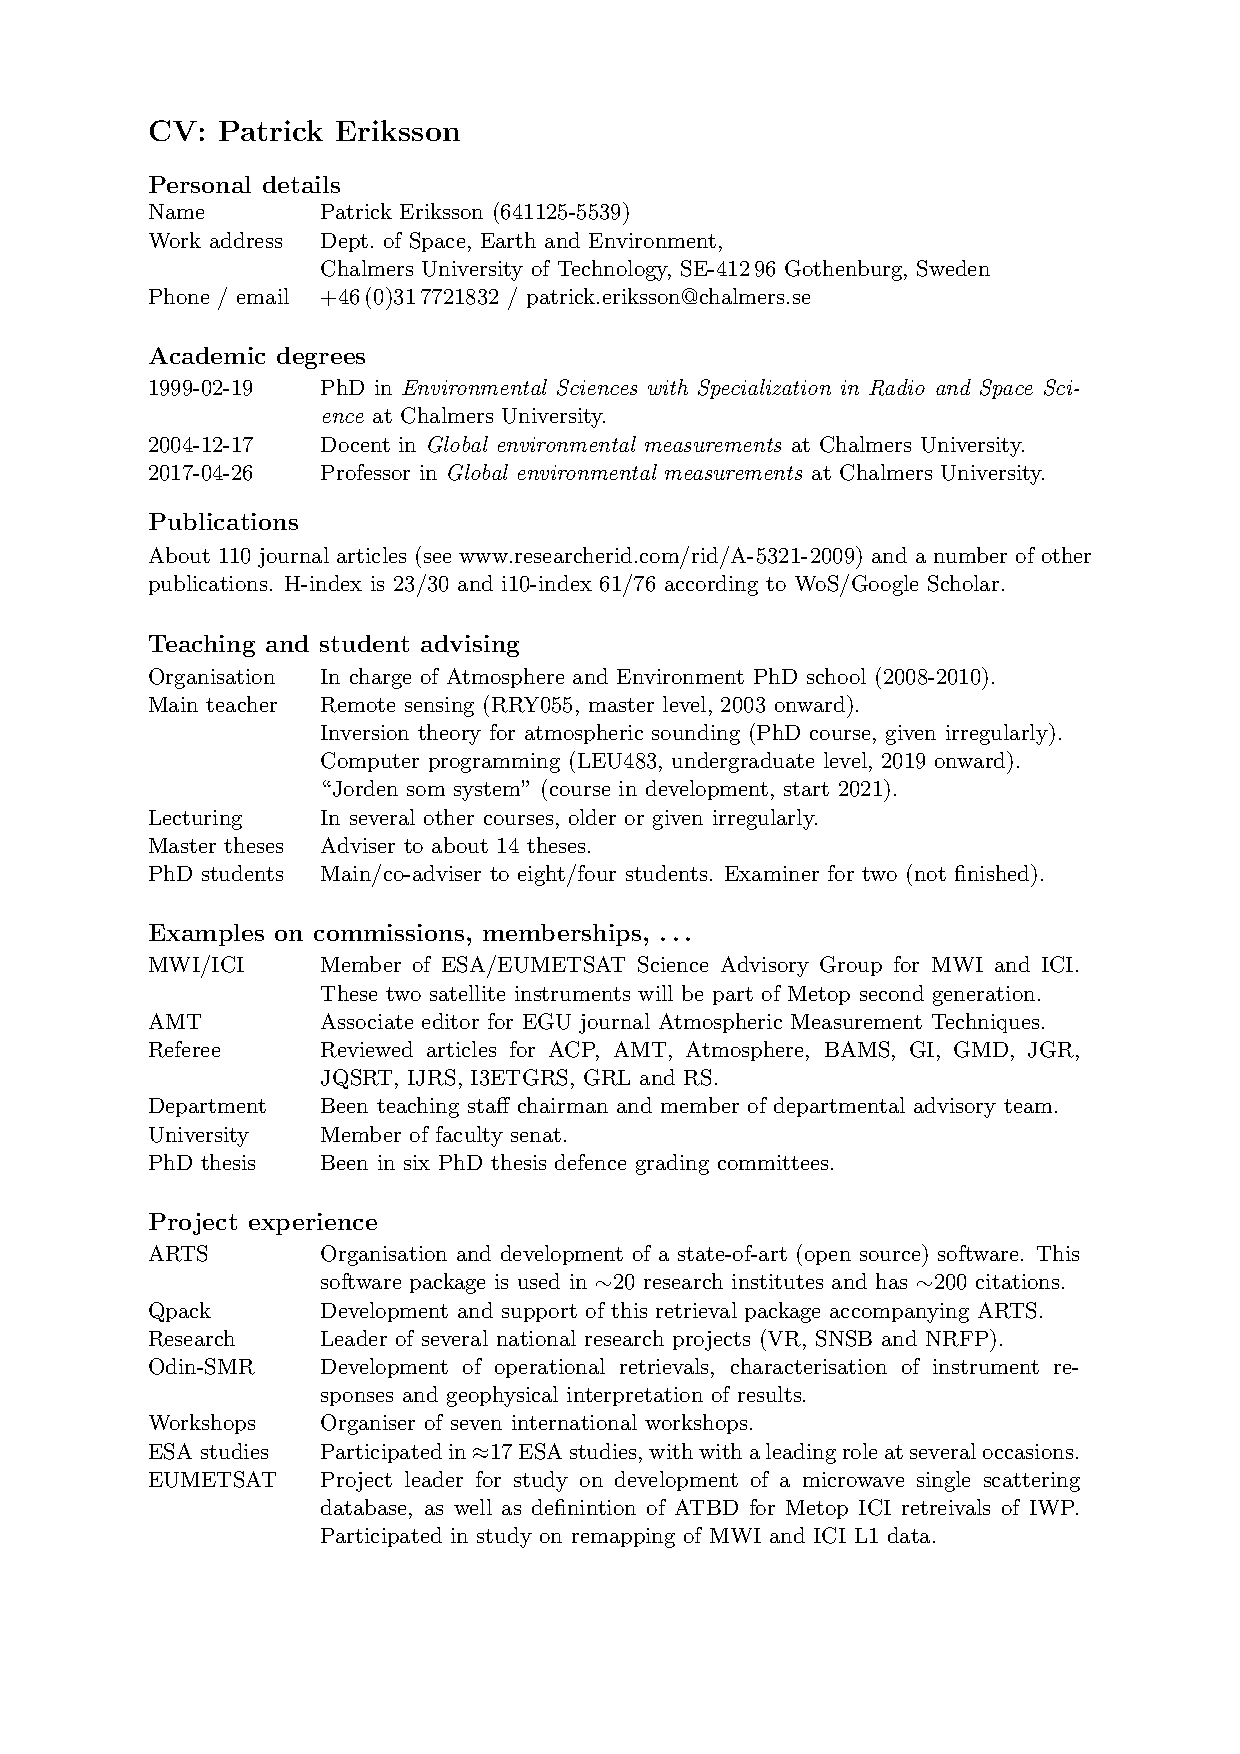
\includepdf[pages={1}]{cv_pe_1page}

\includepdf[pages={1}]{CV_IKaur_1Page}


\end{document}
